
\begin{frame}{Production}
  \begin{minipage}[c][\textheight]{0.45\textwidth}
    \begin{itemize}
      \item 4-top production can proceed through either
        \begin{itemize}
          \item<2,5-> $\mathcal{O}(\alpha_S^4)$ QCD Process
          \item<3,5-> $\mathcal{O}(\alpha_S^2 y_t^2)$ Higgs Exchange
          \item<4,5-> $\mathcal{O}(\alpha_S^2\alpha^2)$ Electroweak Process
        \end{itemize}
      \item<5-> Higgs Exchange + EW gives $\approx10\%$ contribution to total cross-section.
    \end{itemize}
  \end{minipage}
  \begin{minipage}[c][\textheight]{0.45\textwidth}
    \centering
    \only<2>{%
      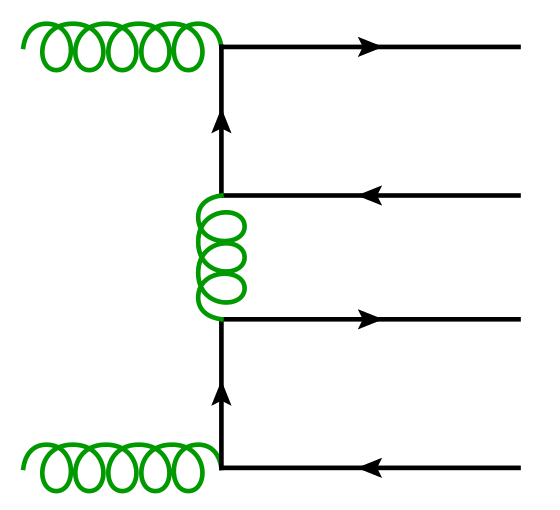
\includegraphics[width=\textwidth]{figures/production-qcd}
    }
    \only<3>{%
      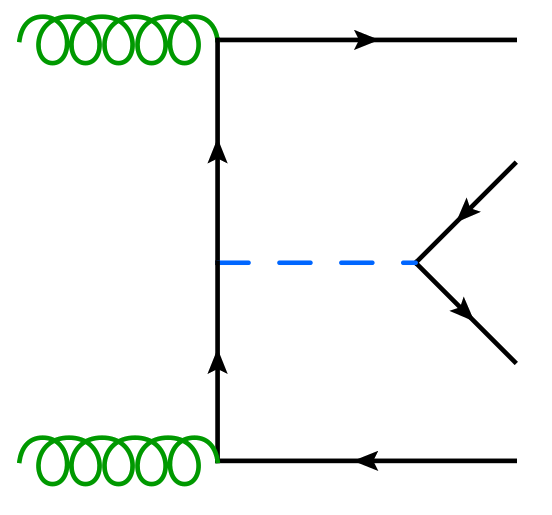
\includegraphics[width=\textwidth]{figures/production-higgs}
    }
    \only<4>{%
      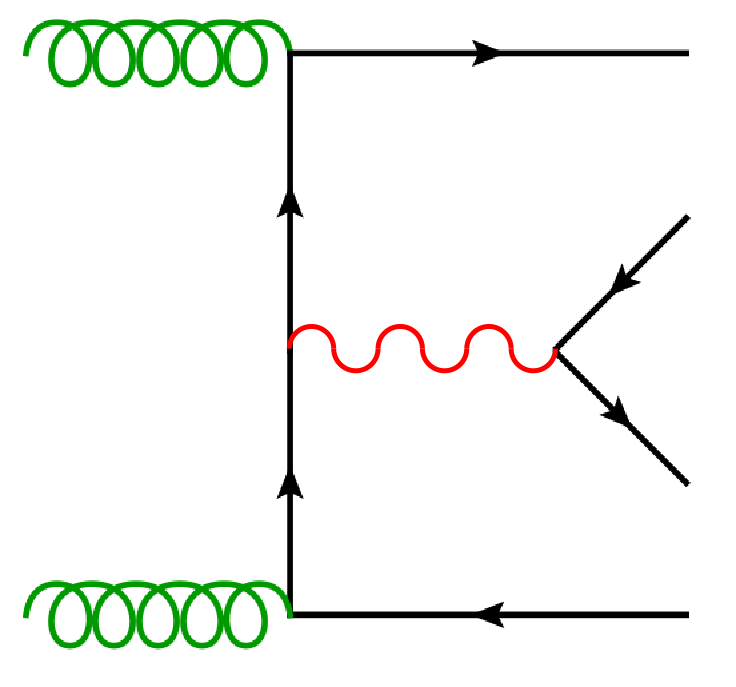
\includegraphics[width=\textwidth]{figures/production-ew}
    }
    \only<5>{%
      Standard Model cross-section at $\sqrt{s}=13\mathrm{TeV}$:
      \begin{center}
        \Huge{12.32\fb{} \MVAt{} NLO}
      \end{center}
    }
    \only<6->{%
      Standard Model cross-section at $\sqrt{s}=13\mathrm{TeV}$:
      \vspace{-.15in}
      \begin{center}
        \Large{12.32\fb{} \MVAt{} NLO}
      \end{center}
      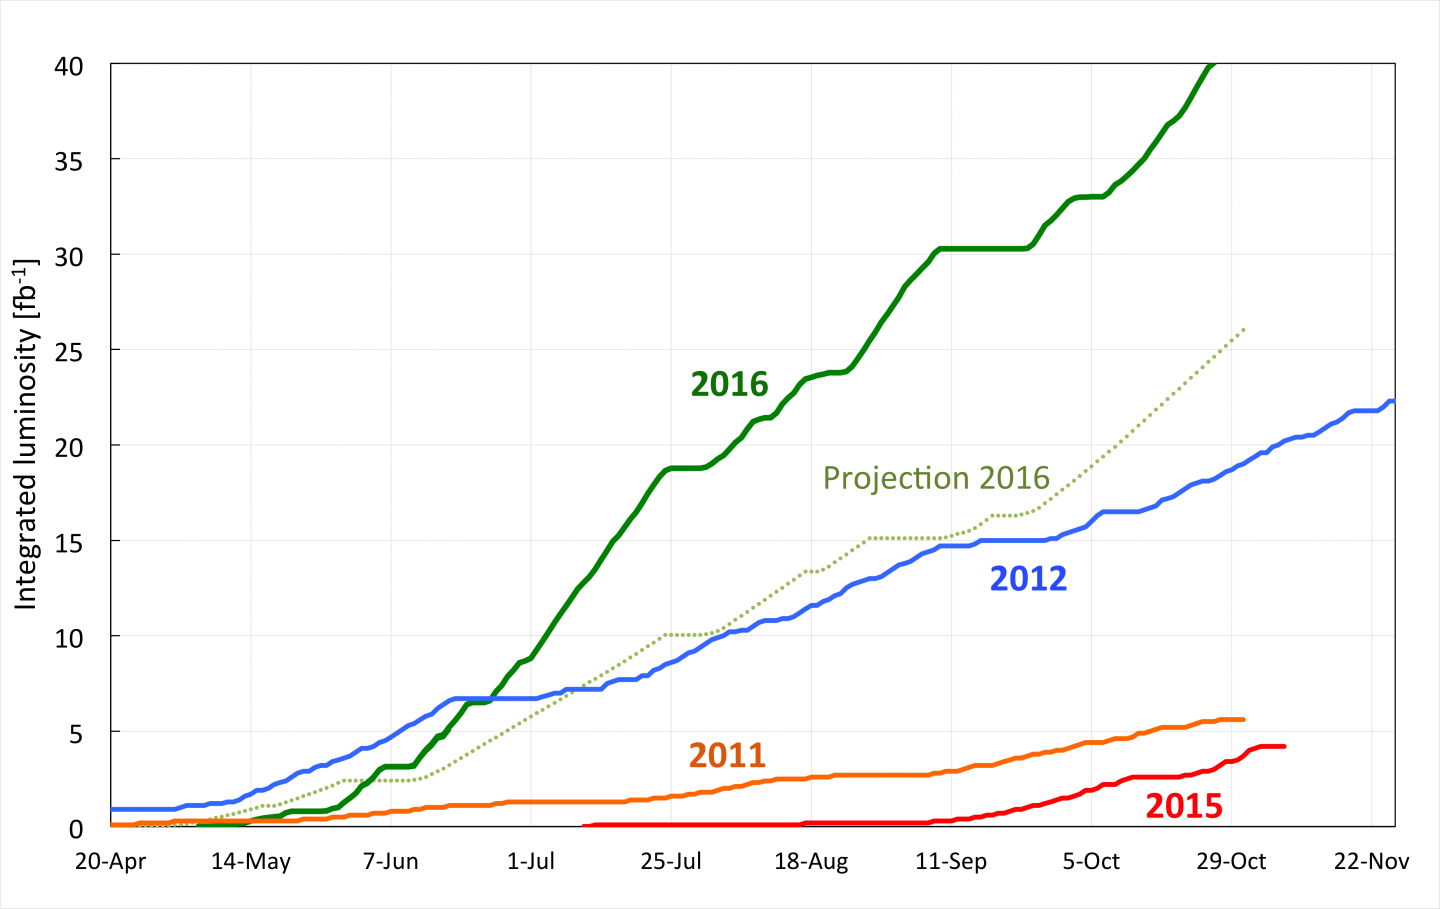
\includegraphics[width=\textwidth]{figures/lhc-luminosity-2016}
      % IMGSRC: https://home.cern/cern-people/updates/2016/12/lhc-report-far-beyond-expectations
      \vspace{-.15in}
      \begin{equation*}
        \mathrm{\#\ Signal\ Events}=12.32\fb * 40\invfb \approx 493
      \end{equation*}
    }
  \end{minipage}
\end{frame}
